%This is chapter 1
%%=========================================
\chapter[Introductions]{Introduction}
\section{Background}
Computer graphics (CG) studies methods for digitally synthesizing and manipulating visual content. An important part of CG is the study of algorithms. This forms the basis for many of the powerful graphics technologies available. One of these technologies is WebGL, a relatively new technology for displaying graphics in web browsers. Since its introduction, the graphical user-experience for the large user mass of the web has been significantly expanded. It allows for almost desktop like graphics performance. 

WebGl has especially expanded the abilities regarding the creation of web browser games and simulations. Creating high performance graphics applications in the browser has never been easier. It has opened up for a sea of possibilities where only one's imagination is the limit.

In a lot of simulation software, and even some games, volumetric information plays a crucial part. With everything from fluid dynamics to voxel games like Minecraft, volumetric information is often a key component~\cite{fluid-simulations-voxel-engine}. One way to acquire such volumetric data is through voxelizing a 3D model (polygon mesh). Voxelization is the process of converting 3D models into a volumetric data. However, to the best of my knowledge, it does not exist any easy-to-use open-source voxelization software written in JavaScript. In order to obtain such volumetric data, developers are therefore forced to go through tedious preprocessing steps, often involving old and complex, hard to use, platform specific tools (for example binvox \cite{binvox}).

This was a problem I encountered myself a year ago in 2019. In connection with an assignment in a simulation course at the Norwegian University of Science and Technology (NTNU), I needed to be able to easily generate some volumetric data based on 3D models. I was using web-technologies, so I was looking for a simple solution in plain JavaScript. However, I was not able to find such a solution. I therefore decided to make one myself. The result was an open-source voxelization engine, written entirely in JavaScript. It was named Voxelizer. The engine is able to load a 3D model and voxelize it.

However, the Voxelizer engine carries strong signs of the limited amount of time allocated for creating the software. By improving and expanding the capabilities of the project, it could serve to be a valuable open-source asset to the web based game- and simulation-development ecosystem, providing easy access to voxelization.

%==========================================
\section{Problem Formulation}

\subsubsection{Problems to be addressed}
There exists an open-source JavaScript voxelization engine for voxelizing 3D models, named Voxelizer. The software faces several issues and is lacking important features. It does not produce accurate and representative results. The output sometimes contains holes and a lot of artifacts. Importing and exporting support is extremely limited. Documentation is lacking, and the coding is of poor quality. The project needs to be professionalized, and made easy to both use and maintain. A more complete description of the problems Voxelizer v0.1.3 faces are described in Section \ref{sec:voxelizer-v013}.

Packaging and publication of new releases, as well as documentation, are tedious and manual procedures. This workflow is prone to human errors, potentially introducing critical bugs. These processes could be automated with modern continuous integration and continuous deployment tools, effectively eliminating these vulnerabilities.

%%=========================================
\section{Objectives}
The main goal of this thesis is to improve and extend the open-source JavaScript Voxelizer engine, turning it into a maintainable and high-quality open-source project. A second goal is to develop complimentary software for the Voxelizer project. This will be in the form of a cross platform desktop application and command line interface (CLI), based on the Voxelizer engine, making it easy to voxelize 3D models.

In order to ensure the maintainability of the various software projects, automation is a critical component. Therefore a third goal is to automate the various software projects as much as possible. This also includes the develop a GitHub Action for automating the API documentation generation process.

%%=========================================
\section{Scope}
The main purpose of this project is to make it easy to conduct high quality voxelization of 3D models. Its scope is limited by the requirements specification defined in the Preliminary report. Complementary to these requirements, a backlog with user-stories has been created. See Appendix~\ref{appendix:backlog}.

It is important to note that the project does not primarily focus on speed of the voxelization algorithm. The targeted systems often run in an environment where resources are scarce. Performance is therefore of course important. However, usability is also extremely important. This thesis will mainly focus on providing easy access to high-quality voxelization, with reasonable performance. If speed is of the main concerns, it would be better to do the extra work of setting up a native solution (for example binvox~\cite{binvox}), often written in C/C++.

%%=========================================
\section{Systems overview}
This section provides an overview of the different repositories developed in connection with this thesis.
\subsection{Voxel systems}
The diagram in Figure~\ref{fig:voxel-systems-overview} shows how the different software repositories regarding voxelization interconnects. The green boxes represents the main software projects developed in conjunction with this thesis. During development, some components were generalized and extracted into a separate repository. This side project is represented by the blue box. The white box represents a third party library.
\begin{figure}[ht]
    \centering
    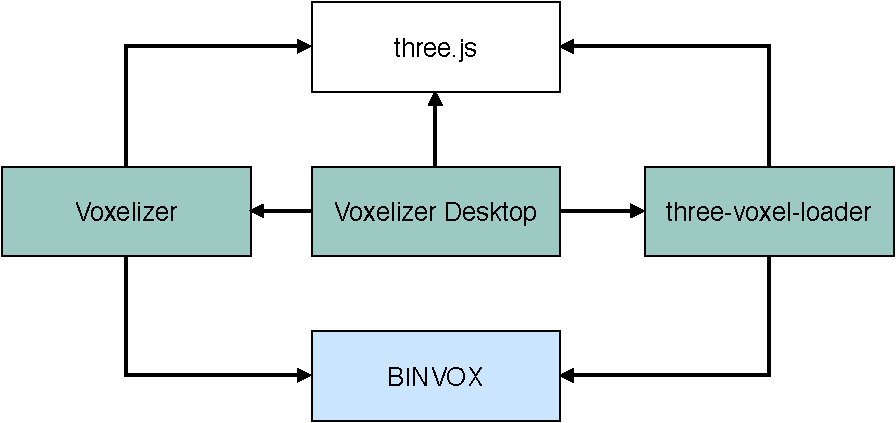
\includegraphics[page=1,scale=0.85]{sections/introduction/figures/voxel-systems-overview.pdf}
    \caption{Voxel systems overview.}
    \label{fig:voxel-systems-overview}
\end{figure}

\subsection{Automation systems}
Figure~\ref{fig:automation-systems-overview} shows a diagram of the various automation repositories. This is mainly GitHub Actions, published to the GitHub Marketplace. The yellow box represents a main project. Throughout the project, it also became clear that some supportive actions needed to be created. These side projects are represented by the blue boxes. The white box represents third party software.
\begin{figure}[ht]
    \centering
    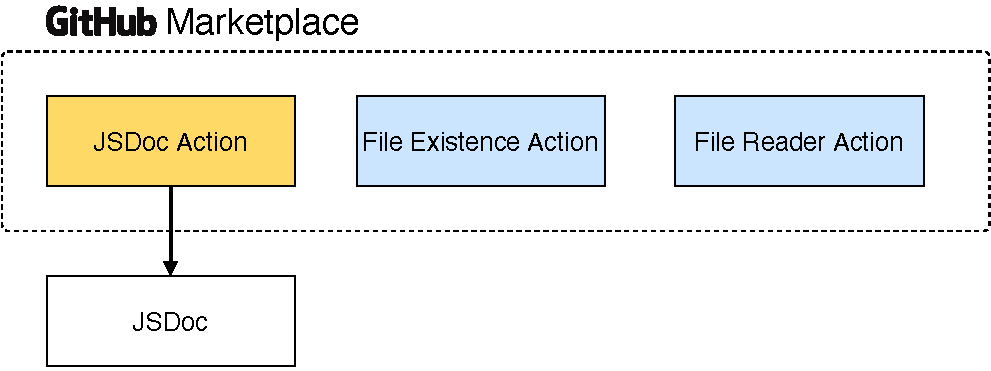
\includegraphics[page=1,scale=0.85]{sections/introduction/figures/automation-systems-overview.pdf}
    \caption{Automation systems overview.}
    \label{fig:automation-systems-overview}
\end{figure}

%%=========================================
\section{Outline}

The rest of the report is structured as follows.\\
\textbf{Chapter 2 - Theory:} Gives an introduction to the theoretical background that lies the foundation of this thesis.\\
\textbf{Chapter 3 - Method:} Contains a description of the methodology and materials used throughout the project.\\
\textbf{Chapter 4 - Result:} Contains a description of the completed works.\\
\textbf{Chapter 5 - Discussion:} Discusses the achieved results, the execution of methodologies, and how the projects could be further improved.\\
\textbf{Chapter 6 - Conclusions:} An overall conclusion of the project is presented, reviewing the objectives and the progress made.